\chapter{Modeling}

\section{Select Modeling Tecnique}

\subsection{Modeling Technique}
% Document the modeling technique that you’ll be using
Random Forest Tree: Random forest is an ensemble learning method for classification, regression and other tasks that operate by constructing a multitude of decision trees at training time and outputting the class that is the mode of the classes (classification) or mean prediction (regression) of the individual trees. Random forest is known for its accuracy and robustness to noise and outliers.

Neural Network: Neural networks are a set of algorithms that are modeled after the human brain and are designed to recognize patterns. Neural networks are used for image recognition, speech recognition, natural language processing, and many other applications. Neural networks are known for their ability to learn from data and generalize to new data.

Adaboost: AdaBoost is an ensemble learning method that combines multiple weak classifiers to create a strong classifier. AdaBoost is used for classification problems and is known for its high accuracy and robustness to noise.

Naive Bayes: Naive Bayes is a probabilistic algorithm that is based on Bayes’ theorem. Naive Bayes is used for classification problems and is known for its simplicity and speed.

Decision Tree: A decision tree is a supervised learning algorithm that is used for classification and regression modeling. It is a method used for predictive modeling, so these trees are used to either classify data or predict what will come next. Decision trees in machine learning can either be classification trees or regression trees. 

\subsection{Modeling Assumptions}
% Record any assumptions about the data that are necessary for the modeling techniques
Random Forest Tree: Random forest assumes that the data is independent and identically distributed (i.i.d.) and that there are no missing values in the data.

Neural Network: Neural networks assume that the data is linearly separable and that there are no missing values in the data.

Adaboost: AdaBoost assumes that the data is i.i.d. and that there are no missing values in the data.

Naive Bayes: Naive Bayes assumes that the features are independent of each other and that there are no missing values in the data.

Decision Tree: Decision tree is a non-statistical approach that makes no assumptions of the training data or prediction residuals; e.g., no distributional, independence, or constant variance assumptions.


\section{Generate Test Design}

\subsection{Test Design}
% Describe how to divide the available dataset into training, test and validation datasets
Generating a test design is an important step in evaluating the performance of modeling techniques. To generate a test design, one needs to define the objective and scope of the test, select the test data, define the performance metrics, and define the procedure for conducting the test.

\section{Build Model}  

\subsection{Random Forest Tree}



We used the sklearn.ensemble library for the Random Forest Tree model. We also employed 5-fold cross-validation to train the model. Finally, we saved the best model out of five and used it for evaluation.
We evaluated the model using different criteria and plotted the Confusion Matrix on Figure \ref{cmRFT}. The table \ref{tableRFT} shows the scores for each criterion.
  

\begin{table}[H]  \centering  
    \begin{tabular}{@{}lllll@{}}
    \toprule
    \multicolumn{5}{c}{Random Forest Tree}                 \\ \midrule
    \multicolumn{5}{l}{Accuracy: 0.8767123287671232}       \\\midrule
                 & precision & recall & f1-score & support \\
    HIGH         & 0.90      & 0.47   & 0.62     & 19      \\ 
    LOW          & 0.86      & 0.96   & 0.91     & 125     \\
    MEDIUM       & 0.89      & 0.86   & 0.88     & 148     \\
    accuracy     &           &        & 0.88     & 292     \\
    macro avg    & 0.88      & 0.76   & 0.80     & 292     \\
    weighted avg & 0.88      & 0.88   & 0.87     & 292     \\ \bottomrule
    \end{tabular}
    \caption{Classification Report of Random Forest}
    \label{tableRFT}
\end{table}


\begin{figure}[H]
    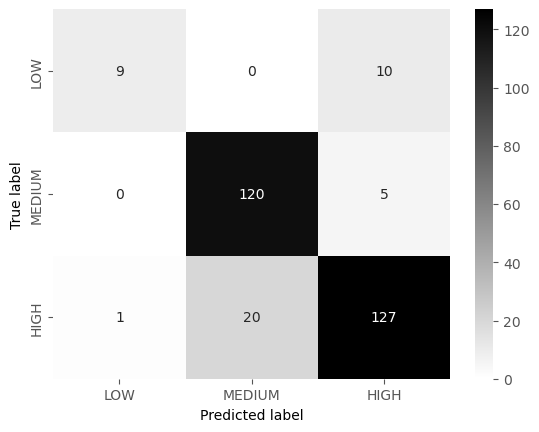
\includegraphics[scale=0.7]{imgs/rft_cm.png}
    \centering
    \caption{Confusion Matrix of Random Forest Tree}
    \label{cmRFT}
\end{figure}


\subsection{Neural Network}

As for Neural Network, We choose the library of MLPClassifier which is part of the Scikit-learn library in Python , The MLPClassifier is a neural network algorithm used for classification tasks. Some parameters are used in this model. The hidden\_layer\_sizes parameter specifies the number of neurons in each layer of the neural network. In this case, there are two hidden layers with 5 neurons each. The activation parameter specifies the activation function used in each neuron. In this case, the ReLU activation function is used. The random\_state parameter is used to initialize the random number generator for reproducibility. The alpha parameter is used for regularization to prevent overfitting. The max\_iter parameter specifies the maximum number of iterations for the solver to converge. The solver parameter specifies the optimization algorithm used to minimize the loss function. In this case, the stochastic gradient descent (SGD) algorithm is used. The tol parameter specifies the tolerance for stopping criteria. The learning\_rate\_init parameter specifies the initial learning rate used by the optimizer 1. 
Here also plot the confusion Matrix \ref*{cmNN} and the result of evaluated table \ref*{tableNN}.


\begin{table}[H]\centering
    \begin{tabular}{@{}lllll@{}}
    \toprule
    \multicolumn{5}{c}{Neural Network}                 \\ \midrule
    \multicolumn{5}{l}{Accuracy: 0.84}       \\\midrule
                 & precision & recall & f1-score & support \\
    HIGH         & 0.56      & 0.72   & 0.63     & 25      \\ 
    LOW          & 0.82      & 0.90   & 0.86     & 173     \\
    MEDIUM       & 0.89      & 0.80   & 0.84     & 240     \\
    accuracy     &           &        & 0.84     & 438     \\
    macro avg    & 0.76      & 0.81   & 0.78     & 438     \\
    weighted avg & 0.84      & 0.84   & 0.84     & 438     \\ \bottomrule
    \end{tabular}
    \caption{Classification Report of Neural Network}
    \label{tableNN}
\end{table}

\begin{figure}[H]
    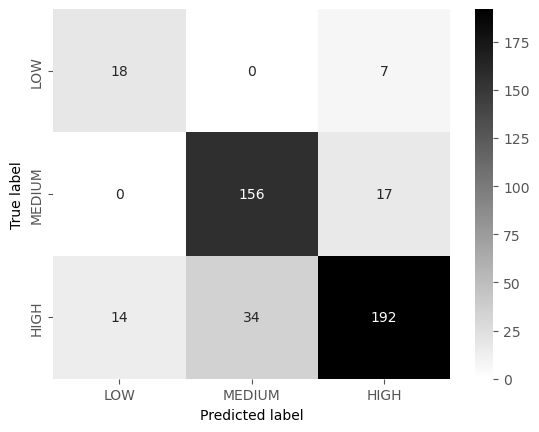
\includegraphics[scale=0.7]{imgs/nn_cm.png}
    \centering
    \caption{Confusion Matrix of Neural Network}
    \label{cmNN}
\end{figure}

\subsection{AdaBoost}

For the AdaBoostClassifier, it is an ensemble learning method that combines multiple weak learners to create a strong classifier. The n\_estimators parameter specifies the number of weak learners to train iteratively. The learning\_rate parameter contributes to the weights of weak learners and uses 1 as a default value.
The Confusion Matrix shows at \ref*{cmadb} and the evaluation table shows at \ref*{tableADB}.

\begin{table}[H]\centering
    \begin{tabular}{@{}lllll@{}}
    \toprule
    \multicolumn{5}{c}{Adaboost}                 \\ \midrule
    \multicolumn{5}{l}{Accuracy:  0.8333333333333334}       \\\midrule
                 & precision & recall & f1-score & support \\
    HIGH         & 0.61      & 0.76   & 0.68     & 25      \\ 
    LOW          & 0.80      & 0.90   & 0.85     & 173     \\
    MEDIUM       & 0.89      & 0.79   & 0.84     & 240     \\
    accuracy     &           &        & 0.11     & 438     \\
    macro avg    & 0.77      & 0.82   & 0.79     & 438     \\
    weighted avg & 0.84      & 0.83   & 0.83     & 438     \\ \bottomrule
    \end{tabular}
    \caption{Classification Report of Adaboost}
    \label{tableADB}
    \end{table}

    \begin{figure}[H]
        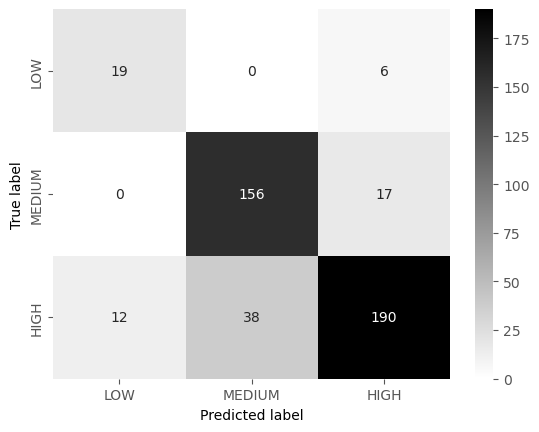
\includegraphics[scale=0.7]{imgs/adb_cm.png}
        \centering
        \caption{Confusion Matrix of Adaboost}
        \label{cmadb}
    \end{figure}


\subsection{Naive Bayes}

The project also uses the Gaussian Naive Bayes algorithm to train a model on the training data. The Gaussian Naive Bayes algorithm is a type of Naive Bayes algorithm that assumes that all features are independent of each other and follow a Gaussian distribution. It is used for classification problems where the input variables are continuous.

The GaussianNB() function from the sklearn.naive\_bayes module is used to create an instance of the Gaussian Naive Bayes algorithm. The instance is then trained on the training data using the fit() method.

the result of Confusion Matrix\ref*{cmnb} and evaluation table \ref*{tablenb} list here.


\begin{table}[H]\centering
    \begin{tabular}{@{}lllll@{}}
    \toprule
    \multicolumn{5}{c}{Naive Bayes}                 \\ \midrule
    \multicolumn{5}{l}{Accuracy: 0.8427}       \\\midrule
                 & precision & recall & f1-score & support \\
    HIGH         & 0.46      & 0.24   & 0.32     & 25      \\ 
    LOW          & 0.69      & 0.77   & 0.73     & 173     \\
    MEDIUM       & 0.76      & 0.74   & 0.75     & 240     \\
    accuracy     &           &        & 0.72     & 438     \\
    macro avg    & 0.64      & 0.58   & 0.60     & 438     \\
    weighted avg & 0.72      & 0.72   & 0.72     & 438     \\ \bottomrule
    \end{tabular}
    \caption{Classification Report of Naive Bayes}
    \label{tablenb}
    \end{table}




\begin{figure}[H]
    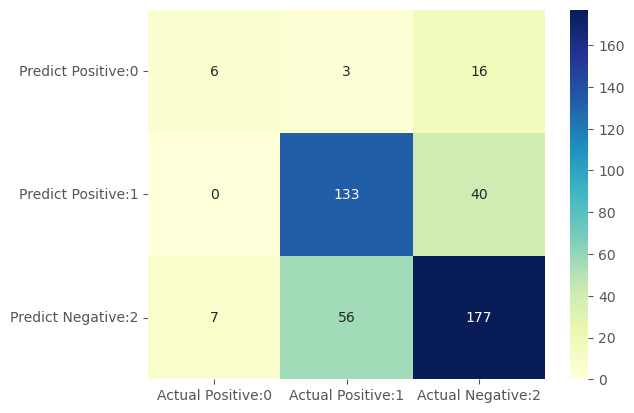
\includegraphics[scale=0.7]{imgs/nb_cm.png}
    \centering
    \caption{Confusion Matrix of Naive Bayes}
    \label{cmnb}
\end{figure}

\subsection{Decision Tree} 

The DecisionTreeClassifier is a class in the sklearn.tree module of the Python Scikit-learn library. It is used to create a decision tree classifier which is a predictive model that can be used for both classification and regression problems. The criterion parameter specifies the function to measure the quality of a split. In this case, we use the supported criteria is “gini” for the Gini impurity.
Confusion Matrix \ref{cmdt} and Classification Report of Decision Tree \ref{tabledt}.
\begin{table}[H]\centering
    \begin{tabular}{@{}lllll@{}}
    \toprule
    \multicolumn{5}{c}{Decision Tree}                 \\ \midrule
    \multicolumn{5}{l}{Accuracy: 0.7990867579908676}       \\\midrule
                 & precision & recall & f1-score & support \\
    HIGH         & 0.49      & 0.68   & 0.57     & 25      \\ 
    LOW          & 0.79      & 0.87   & 0.83     & 173     \\
    MEDIUM       & 0.86      & 0.76   & 0.81     & 240     \\
    accuracy     &           &        & 0.80     & 438     \\
    macro avg    & 0.71      & 0.77   & 0.73     & 438     \\
    weighted avg & 0.81      & 0.80   & 0.80     & 438     \\ \bottomrule
    \end{tabular}
    \caption{Classification Report of Decision Tree}
    \label{tabledt}
    \end{table}

    \begin{figure}[H]
        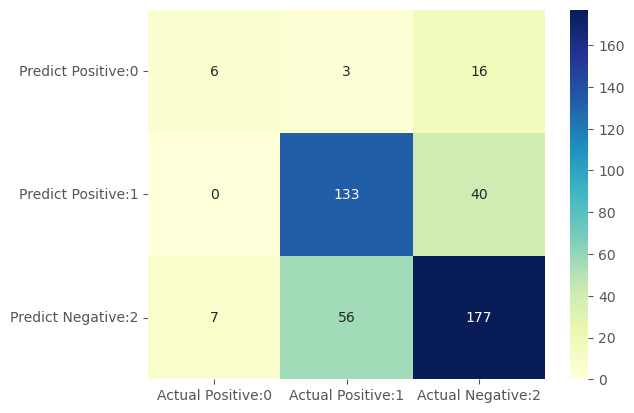
\includegraphics[scale=0.7]{imgs/nb_cm.png}
        \centering
        \caption{Confusion Matrix of Decision Tree}
        \label{cmdt}
    \end{figure}